        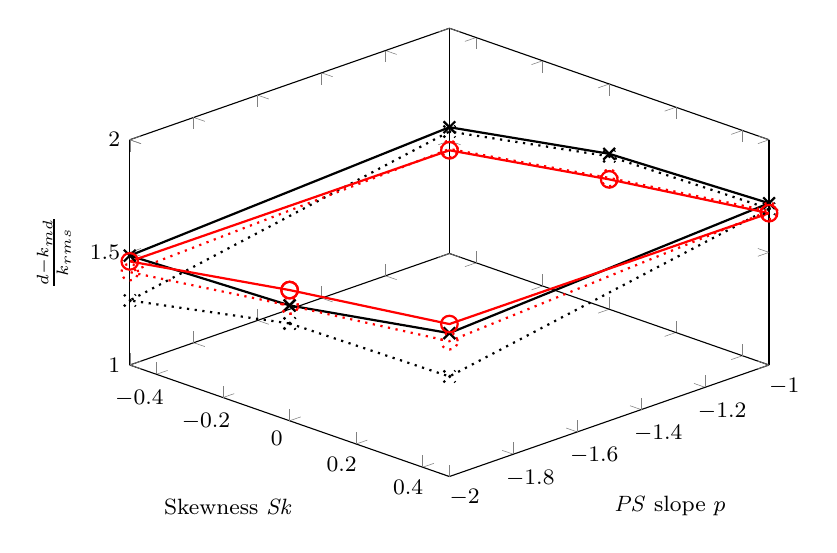
\begin{tikzpicture}[]
        \centering
        \begin{axis}[
        view={45}{35},
            ylabel={\textit{PS} slope $p$},
            xlabel={Skewness \textit{Sk}},
			zlabel={$\frac{d-k_{md}}{k_{rms}}$},
		%	ztick={5.5,6,6.5,7,7.5},
            zmin=1, zmax=2,
            width=.8\textwidth,
            height=.6\textwidth,
            label style={font=\footnotesize},
            tick label style={font=\footnotesize}
            ]

                        \addplot3 [
            black,mark=x,thick, mark size=3pt
            ]
            coordinates{
            (0,-2,0.03024/0.02)			
			(0.48,-2,0.03404/0.0208)
			(0.48,-1,0.03574/0.0208)
			(0,-1,0.0338/0.02)
			(-0.48,-1,0.03246/0.0208)
			(-0.48,-2,0.0309/0.0208)
            (0,-2,0.03024/0.02)
			};
			\addplot3 [
            black,dotted,mark=x,thick, mark size=3pt
            ]
            coordinates{
            
            (0,-2,0.02864/0.02)
			(0.48,-2,0.03004/0.0208)
			(0.48,-1,0.03524/0.0208)
			(0,-1,0.03358/0.02)
			(-0.48,-1,0.03206/0.0208)
			(-0.48,-2,0.02676/0.0208)
			(0,-2,0.02864/0.02)
            };
            
            
            
            
                                    \addplot3 [
            red,mark=o,thick, mark size=3pt
            ]
            coordinates{
            (0,-2,1.58018)			
			(0.48,-2,1.6769)
			(0.48,-1,1.67396)
			(0,-1,1.57652)
			(-0.48,-1,1.45811)
			(-0.48,-2,1.45994)
            (0,-2,1.58018)
			};
			\addplot3 [
            red,mark=o,dotted,thick, mark size=3pt
            ]
            coordinates{
            
            (0,-2,1.51138)
			(0.48,-2,1.6007)
			(0.48,-1,1.68346)
			(0,-1,1.58295)
			(-0.48,-1,1.46401)
			(-0.48,-2,1.41258)
			(0,-2,1.51138)
            };
        \end{axis}
        \end{tikzpicture}